\chapter{Foundations}
\label{ch:foundations}

In this chapter it is important to first evaluate why data sovereignty cannot be
established by the location of a data centre alone. We therefore explore the
various conceptual, legal and technical foundations on which the evaluation in
the following chapters depends.

We begin in \cref{sec:sovereignty-definition} by defining data sovereignty and
separating it from the terms with which it is commonly conflated. In
\cref{sec:legal-landscape} we explore the European and United States legal
instruments that determine which jurisdiction may compel access to cloud-hosted
data. \Cref{sec:full-stack} then extends the question from law to system
architecture, showing that sovereignty claimed at one layer of a platform
depends on the layers beneath it, and \cref{sec:technical-foundations}
introduces the virtualization and platform concepts on which the benchmarking
study in \cref{sec:method-study4} relies. Finally, \cref{sec:related-work}
reviews related work.

\section{Data Sovereignty: Definition and Dimensions}
\label{sec:sovereignty-definition}

The term \emph{data sovereignty} is used in more than one sense. In vendor
literature it most often refers simply to the country in which data is stored.
In European policy it carries a broader industrial meaning, covering not only
the confidentiality of European data but also the competitiveness of European
providers and the reduction of strategic dependency on foreign vendors
\cite{Blancato_CloudSovereigntyNexus_2024}. The two senses can lead to opposite
conclusions about the same provider, and so we fix the terminology here before
applying it to any assessment.

\subsection{Four Distinct Properties}
\label{subsec:four-properties}

Four properties are commonly grouped together under the heading of sovereignty.
They are not the same thing, and a provider may satisfy one while failing the
others. \Cref{tab:sovereignty-dimensions} sets out the distinction.

\begin{table}[htbp]
  \centering
  \caption{Four properties commonly grouped under the term
           \enquote{sovereignty}, the question each answers, and what actually
           determines it.}
  \label{tab:sovereignty-dimensions}
  \small
  \begin{tabularx}{\textwidth}{@{}l X l@{}}
    \toprule
    \textbf{Property} & \textbf{Question it answers} & \textbf{Determined by} \\
    \midrule
    Data residency
      & In which territory is the data stored and processed?
      & Facility location \\[0.4em]
    Data sovereignty
      & Which jurisdiction may lawfully compel its disclosure?
      & Corporate incorporation \\[0.4em]
    Operational sovereignty
      & Who is technically able to access or administer the system?
      & Staffing and key control \\[0.4em]
    Technological sovereignty
      & Can the stack be inspected, modified and operated independently?
      & Supply chain and licensing \\
    \bottomrule
  \end{tabularx}
\end{table}

\textbf{Data residency} concerns geography alone. It is satisfied when storage
and processing occur within a defined territory, and it is the property most
easily demonstrated, since a provider can evidence it with a data centre
address.

\textbf{Data sovereignty} concerns jurisdiction: which state may lawfully
compel a provider to disclose customer data. This is determined by the legal
personality of the operating company and of its parent, not by where its
facilities stand. We develop this distinction in
\cref{subsec:location-jurisdiction}.

\textbf{Operational sovereignty} concerns administrative access. A provider
whose support engineers hold privileged access from outside the territory, or
which retains the encryption keys protecting customer data, has not placed that
data beyond external reach even where residency and jurisdiction are both
satisfied.

\textbf{Technological sovereignty} concerns the stack itself: whether the
hardware, firmware and software can be audited, modified and operated without
dependence on a single foreign supplier. We return to this property in
\cref{sec:full-stack}.

\subsection{Why Location Alone Does Not Guarantee Sovereignty}
\label{subsec:location-jurisdiction}

It is often assumed that because data resides in a given geographical location,
it is beyond the reach of foreign jurisdiction. The assumption does not hold
where the law of a provider's country of incorporation reaches the conduct of
its subsidiaries overseas. A data centre in Frankfurt operated by the European
subsidiary of a company incorporated in the United States satisfies residency
completely, but the parent company remains subject to disclosure obligations under
United States law that can reach data held abroad.

This is not just a theoretical concern, but a legitimate one. In December 2013 federal agents applied to
the District Court for the Southern District of New York for a warrant under the
Stored Communications Act, requiring Microsoft to disclose the contents of a
customer's electronic mail account in an investigation into illegal drug
trafficking \cite{MicrosoftIreland_SCOTUS_2018}. Microsoft established that the
account's contents were held in a single location, its datacentre in Dublin, and
moved to quash the warrant in respect of that data. The magistrate judge denied
the motion, the District Court affirmed and held Microsoft in civil contempt, and
on appeal the Court of Appeals for the Second Circuit reversed, holding that
compelling disclosure would be an unauthorised extraterritorial application of
the statute \cite{MicrosoftIreland_2dCir_2016}.

The question was never resolved judicially. On 23~March 2018, while the appeal
was pending before the Supreme Court, Congress enacted the \ac{CLOUD Act}
\cite{CLOUDAct_2018}, which amends the Stored Communications Act to require a
provider to preserve, back up or disclose data within its possession, custody or
control \enquote{regardless of whether such communication, record, or other
information is located within or outside of the United States}. The Government
obtained a fresh warrant under the amended statute, and the Supreme Court vacated
the judgment below and remanded with instructions to dismiss the case as moot
\cite{MicrosoftIreland_SCOTUS_2018}.

Residency is therefore a necessary but insufficient condition for sovereignty.
An assessment that treats the two as equivalent will systematically overstate
the sovereignty of providers whose corporate parent lies outside the
\ac{EU}. The legal instruments behind this position are examined in
\cref{sec:legal-landscape}, and its consequences for provider selection are
quantified in \cref{sec:study1}.

\subsection{The Definition Adopted in This Work}
\label{subsec:definition-adopted}

We treat sovereignty as a composite property spanning all four dimensions in
\cref{tab:sovereignty-dimensions}. To operationalise it we adopt the Cloud
Sovereignty Framework \cite{EC_DIGIT_CloudSovereignty_2025}. The framework
decomposes the concept into eight weighted objectives covering strategic,
legal, data, operational, supply-chain, technological, security and
environmental criteria.

We adopt this framework rather than construct our own for two reasons. It is
issued by the institution that defines European public-sector procurement
policy, which makes the resulting scores externally meaningful rather than
particular to this study; and its objectives already separate the four
properties above, so a provider cannot compensate for a jurisdictional weakness
with a strong residency position. Its structure and scoring rules are specified
in \cref{sec:method-study1}.

\section{Legal and Regulatory Landscape}
\label{sec:legal-landscape}

It is important to consider the legal frameworks and regulations that bind the
cloud industry, and how the United States, the European Union, China and other
jurisdictions are each navigating the question of data sovereignty. These
frameworks have developed independently and in pursuit of different aims, and where
they meet they frequently clash: a disclosure that one jurisdiction compels may
be one that another forbids. A provider operating across them is therefore
subject to obligations it cannot fully satisfy at the same time, and an
enterprise selecting that provider inherits the conflict.

Within the European Union the position is complicated further by the form the
legislation takes. A regulation binds every member state directly and
identically, which is how the Union has been able to impose a single data
protection standard across all twenty-seven. A directive sets only the objective
and leaves each member state to give it effect through its own national law, so
that a single European obligation can reach an enterprise in twenty-seven
different forms. Whether a given requirement is uniform or fragmented therefore
depends on the instrument that carries it.

We begin in \cref{subsec:regulations-directives} with the two forms European law
takes, since this determines how every obligation that follows reaches an
enterprise. \Cref{subsec:gdpr-schrems} then examines the European position on
international data transfers, \cref{subsec:cloud-act} the United States
instruments, and \cref{subsec:other-jurisdictions} the Chinese instruments.

\subsection{Regulations versus Directives}
\label{subsec:regulations-directives}

The European Union makes law in two main forms, and the difference between them
decides whether a rule is the same everywhere in Europe or different in each
country. The distinction is worth setting out before any specific law is
discussed, because it determines how each of them actually reaches an
enterprise.

A \textbf{regulation} becomes law in every member state on the day it takes
effect. No national parliament has to act, and no national law has to be
written. The rule that applies in Germany is the same rule, in the same words,
that applies in France and in Ireland.

A \textbf{directive} does not become law by itself. It states a result that
every member state must achieve and sets a deadline by which each must pass its
own national law achieving it. Twenty-seven countries therefore produce
twenty-seven laws. Those laws pursue a common objective, but they can differ in
scope, in detail and in the penalties they impose, and they take effect only
when each country has passed them.

This division is set out in Article~288 of the Treaty on the Functioning of the
European Union, which describes a regulation as \enquote{binding in its entirety
and directly applicable} in all member states, and a directive as
\enquote{binding, as to the result to be achieved} while leaving \enquote{to the
national authorities the choice of form and methods} \cite{TFEU_Art288}.

\Cref{fig:eu-instruments} shows how the two paths differ once an act has been
adopted.

\begin{figure}[htbp]
  \centering
  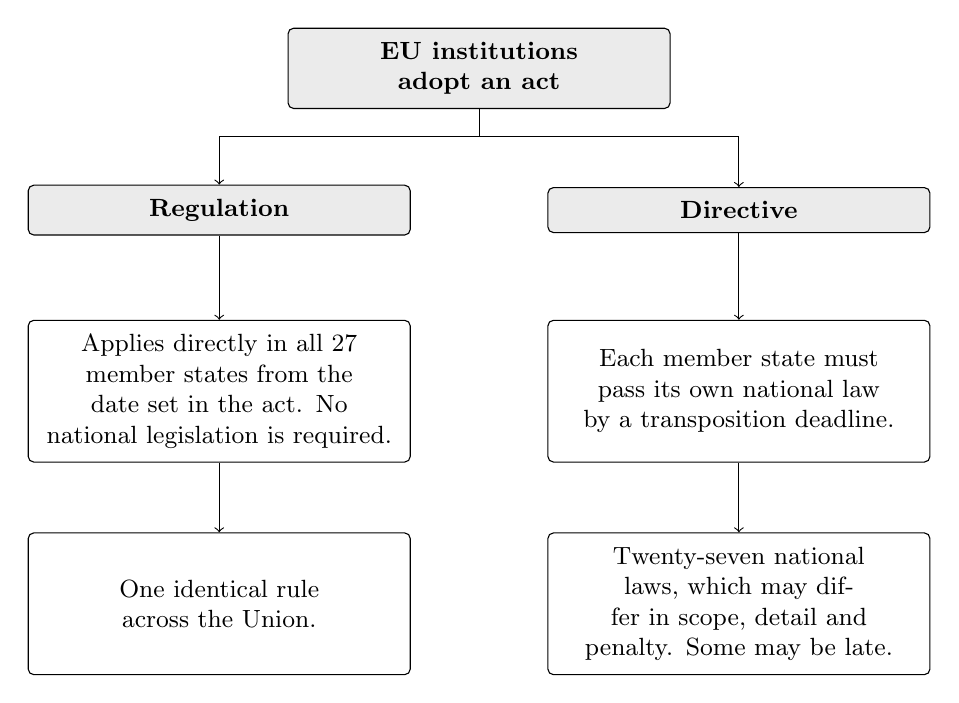
\begin{tikzpicture}[
    box/.style = {draw, rounded corners=2pt, align=center, text width=4.5cm,
                  inner sep=5pt, font=\small, minimum height=1.8cm},
    hdr/.style = {draw, rounded corners=2pt, align=center, text width=4.5cm,
                  inner sep=5pt, font=\small\bfseries, fill=black!8},
  ]
    \node[hdr] (adopt) at (0,0)       {EU institutions adopt an act};
    \node[hdr] (reg)   at (-3.3,-1.8) {Regulation};
    \node[hdr] (dir)   at (3.3,-1.8)  {Directive};
    \node[box] (reg2)  at (-3.3,-4.1) {Applies directly in all 27 member states
                                       from the date set in the act. No national
                                       legislation is required.};
    \node[box] (dir2)  at (3.3,-4.1)  {Each member state must pass its own
                                       national law by a transposition
                                       deadline.};
    \node[box] (reg3)  at (-3.3,-6.8) {One identical rule across the Union.};
    \node[box] (dir3)  at (3.3,-6.8)  {Twenty-seven national laws, which may
                                       differ in scope, detail and penalty.
                                       Some may be late.};

    \draw[->] (adopt.south) -- ++(0,-0.35) -| (reg.north);
    \draw[->] (adopt.south) -- ++(0,-0.35) -| (dir.north);
    \draw[->] (reg.south)  -- (reg2.north);
    \draw[->] (dir.south)  -- (dir2.north);
    \draw[->] (reg2.south) -- (reg3.north);
    \draw[->] (dir2.south) -- (dir3.north);
  \end{tikzpicture}
  \caption{How a regulation and a directive reach a member state.}
  \label{fig:eu-instruments}
\end{figure}

Both forms govern the subject of this thesis, and
\cref{tab:eu-instruments} lists the instruments most relevant to it. The
\ac{GDPR} is a regulation \cite{GDPR2016}, which is why one data protection
standard applies identically across the Union. \Ac{NIS2} is a directive
\cite{NIS2_2022}, and member states were given until 17~October 2024 to pass
their implementing laws. Not all of them did. As of 2026 the Commission has
referred Ireland, Spain, France and the Netherlands to the \ac{CJEU} for failing
to notify the measures transposing it into national law
\cite{EC_NIS2_Status_2026}.

\begin{table}[htbp]
  \centering
  \caption{European instruments governing cloud provision, by form. Only
           \acs{NIS2} is a directive; the remainder apply directly.}
  \label{tab:eu-instruments}
  \small
  \begin{tabularx}{\textwidth}{@{}l l X l@{}}
    \toprule
    \textbf{Instrument} & \textbf{Form} & \textbf{What it governs} & \textbf{Applies from} \\
    \midrule
    \acs{GDPR}
      & Regulation & Protection of personal data and its transfer outside the Union
      & 2018 \\[0.35em]
    \acs{NIS2}
      & \textbf{Directive} & Cybersecurity of network and information systems
      & Transposition due 2024 \\[0.35em]
    \acs{DORA}
      & Regulation & ICT operational resilience in the financial sector; oversight
        of critical ICT third-party providers, cloud providers included
      & 2025 \\[0.35em]
    Data Act
      & Regulation & Access to and use of data; switching between data-processing
        services
      & 2025 \\[0.35em]
    \acs{CRA}
      & Regulation & Cybersecurity requirements for products with digital elements
      & 2027 \\
    \bottomrule
  \end{tabularx}
\end{table}

Two features of \cref{tab:eu-instruments} matter for provider assessment. The
first is that only one of these instruments is a directive, which reflects a
deliberate shift: legislating by regulation is how the Union avoids the
fragmentation the previous subsection described. The second is that two of them
bear directly on the questions this thesis asks. \Ac{DORA} \cite{DORA_2022}
brings critical cloud providers under direct supervisory oversight, and the Data
Act \cite{DataAct_2023} establishes a right to switch between providers, which
speaks to the vendor lock-in examined in \cref{ch:conclusion}. The \ac{CRA}
\cite{CRA_2024} reaches further down the stack, imposing obligations on the
products and components from which infrastructure is built
(\cref{sec:full-stack}).

The consequence for this research is that \enquote{\ac{EU} compliance} is not a
single property that a provider either has or lacks. Where an obligation comes
from a regulation, a provider either meets it or does not, and the answer is the
same across Europe. Where it comes from a directive, what the provider owes
depends on which member states it and its customer operate in, and in some
countries the obligation may not yet be in force at all. Scoring providers on a
single measure of European compliance would conceal that difference, which is
one reason this study assesses them against the Commission's own framework
(\cref{subsec:definition-adopted}) rather than against national implementations
that vary by deployment.

\subsection{GDPR and the Schrems II Ruling}
\label{subsec:gdpr-schrems}

The \ac{GDPR} \cite{GDPR2016} is a regulation, which by the distinction drawn in
\cref{subsec:regulations-directives} means it applies in identical form in every
member state, without any national parliament having to pass a law. It governs
how personal data may be collected, stored and used, and it binds any
organisation processing the personal data of people in the Union, wherever that
organisation is itself established.

One part of it matters particularly here. The Regulation restricts sending
personal data outside the Union. The reason is straightforward: rights that
apply inside Europe would count for little if data could simply be moved to a
country where they do not apply. A transfer abroad is therefore lawful only if
the protection travels with the data.

Chapter~V of the Regulation offers three ways to establish that it does
\cite{GDPR2016}:

\begin{itemize}
  \item an \textbf{adequacy decision}, in which the Commission examines a
        country's laws and finds that they protect personal data to a standard
        comparable with the Union's, after which data may flow there as freely
        as to a member state;
  \item \textbf{appropriate safeguards}, in practice a contract on standard
        clauses published by the Commission, through which the recipient commits
        itself to European standards; or
  \item a \textbf{derogation}, a narrow exception for particular cases such as
        the explicit consent of the person concerned, not intended to carry
        routine transfers.
\end{itemize}

The first two were both tested against United States law, in litigation brought
by a single complainant that ran for most of a decade.

Maximillian Schrems, an Austrian Facebook user, complained to the Irish data
protection authority that his data, sent by Facebook Ireland to servers in the
United States, was not protected against access by United States authorities.
The complaint failed, because the Commission had already found the United States
adequate under an arrangement called Safe Harbour. In 2015 the Court declared
that finding invalid \cite{SchremsI_2015}. Schrems complained again, this time
about transfers made under the standard contractual clauses, and by the time the
case reached the Court the Commission had issued a replacement adequacy
decision: the \ac{EU}--US Privacy Shield.

In 2020 the Court struck that down too \cite{SchremsII_2020}. It gave two
reasons. United States surveillance law let government agencies reach the data
far more freely than European law allows. And a European whose data ended up
there had no practical way to challenge it, because United States courts were
not open to them.

The standard contractual clauses themselves survived. The Court examined them in
the same judgment and left them in place. So after 2020 a company could still
send personal data to the United States under a contract, but it could no longer
rely on the Commission having declared the country safe.

What the judgment exposed matters more than which decision fell. The \ac{GDPR}
binds those who handle personal data: the organisation that decides why it is
processed, the organisation that processes it, and the contract between them. It
does not bind foreign states. Where a destination country's law permits its
authorities to reach data on terms Europe considers disproportionate, neither
the Regulation nor any contract written under it can change that, because a
contract binds only the parties who sign it. This is why the Court invalidated
an adequacy decision rather than ordering a remedy: nobody had breached the
Regulation, and there was nothing within it capable of neutralising a foreign
statute. Its answer was instead to place the burden on the sender, who must
assess the destination country's legal system before transferring and suspend
the transfer where the required protection cannot be guaranteed.

For an enterprise choosing a cloud provider, this means that reading the
contract is not enough. However carefully a contract is written, it cannot stop
a government from ordering the provider to hand data over. The question that
decides the outcome is which country's law the provider is subject to
(\cref{subsec:location-jurisdiction}), and what that law allows the government
to demand. 


\subsection{Extraterritorial Reach: CLOUD Act and FISA 702}
\label{subsec:cloud-act}

United States law gives its government two separate ways to obtain data held by
an American company. They work differently, and treating them as one obscures
which of them actually matters to a European enterprise.
\Cref{tab:us-powers} sets them side by side.

\begin{table}[htbp]
  \centering
  \caption{Two routes by which United States authorities can reach data held by
           an American provider.}
  \label{tab:us-powers}
  \small
  \begin{tabularx}{\textwidth}{@{}l X X@{}}
    \toprule
    & \textbf{\acs{CLOUD Act}} & \textbf{FISA section 702} \\
    \midrule
    Purpose          & Criminal investigation & Foreign intelligence \\[0.35em]
    Who is targeted  & A named account in a specific case
                     & People who are not United States citizens and are
                       outside the United States \\[0.35em]
    Customer informed & Sometimes & No \\[0.35em]
    Provider can contest & Yes, in open court & Limited, and in secret \\
    \bottomrule
  \end{tabularx}
\end{table}

The first route is the \ac{CLOUD Act}, already described in
\cref{subsec:location-jurisdiction}. It serves criminal investigation. A
prosecutor obtains a warrant for a named account and the provider must produce
what it holds. The provider knows the order exists and can challenge it in
court, as Microsoft did.

The second is section~702 of the Foreign Intelligence Surveillance Act
\cite{FISA702}. It serves intelligence collection rather than prosecution. It
authorises surveillance of people who are not United States citizens and are
believed to be outside the United States, and it compels providers to assist.
The provider is not permitted to tell the affected customer.

For a European enterprise the second matters more than the first, for a
straightforward reason: a European company, employees and customers are precisely the
people section~702 is aimed at. They are not United States citizens and they are
not in the United States. A criminal warrant is an exceptional event that may
never arrive; falling inside the target group of a foreign intelligence
programme is a permanent condition.

\subsubsection*{The test is control, not location}

Neither power depends on where the servers stand. The \ac{CLOUD Act} reaches
data within a provider's possession, custody or control --- a test about what
the company is able to obtain, not about where it is kept. If an American parent
can instruct its European subsidiary to retrieve data, or holds credentials that
reach into that subsidiary's systems, the data is within its control.

This is why establishing a European subsidiary does not by itself solve the
problem. What decides the question is the ownership chain and the access paths:
who can instruct whom, and which staff and systems can reach the data. A
subsidiary wholly owned by an American parent, administered by staff who
ultimately report to it, or dependent on its systems for support and
maintenance, remains within reach.

\subsubsection*{Where the two legal systems collide}

European law anticipated this situation. Under the \ac{GDPR}, an order from a
foreign court or government agency demanding personal data is not by itself a
lawful reason for a European company to hand it over \cite{GDPR2016}. The order
counts only if the two countries have a treaty covering requests of that kind.
Such treaties exist, and they work by sending the request from one government to
the other, which then obtains the data through its own courts.

A warrant served directly on the provider skips that route entirely. Under
European law it is therefore not a valid reason to disclose anything.

A provider caught by both systems is then stuck. American law tells it to hand
the data over. European law tells it the order is not a reason to do so.
Whichever it obeys, it breaks the other, and neither the provider nor its
customer can resolve that.

The consequence for this thesis is the assessment criterion itself. A provider
cannot be judged on where its data centres are, because neither power turns on
that. It has to be judged on where it is incorporated, who owns it, and who can
reach its systems --- which is what the sovereignty instrument described in
\cref{sec:method-study1} sets out to measure.


\subsection{China and Other Jurisdictions}
\label{subsec:other-jurisdictions}

The previous subsection might suggest a simple remedy: avoid American providers.
It is not that simple. Other countries have their own rules about data crossing
their borders, and those rules do not all point the same way.

China restricts data leaving the country in much the same way Europe does. Under
its Data Security Law, data held in China may not be handed to a foreign law
enforcement authority unless the Chinese government approves
\cite{ChinaDSL_2021}. Its Personal Information Protection Law says the same for
personal data \cite{ChinaPIPL_2021}. The reasoning is the one already seen in
\cref{subsec:cloud-act}: a country that has gone to the trouble of regulating
data held on its territory does not want a foreign government reaching past it.

The pattern is worth noticing. Europe and China have arrived at the same
position, and neither will let a company hand data to a foreign government
without going through an agreed channel. The United States is the outlier, with
a law that reaches the other way. A provider operating in all three is caught
between rules that were built to resist one another.

China also has a law on cooperation with intelligence work. It requires an
organisation to support, assist and cooperate in national intelligence work
\enquote{in accordance with the law}, and a later provision states that such
work must respect human rights and protect the lawful rights and interests of
organisations \cite{ChinaNIL_2017}. How far the obligation reaches in practice
is disputed, and the qualifying words are often dropped when the provision is
quoted. This thesis takes no position on that dispute. What matters for an
assessment is that the obligation exists and that its limits are not settled.

None of the providers assessed in this thesis is Chinese-owned, so the question
does not arise through ownership. It arises through equipment. A European
provider that builds its infrastructure on hardware and firmware manufactured
elsewhere inherits whatever questions attach to that equipment, and it cannot
answer them by pointing at its own place of incorporation. This is the
supply-chain side of sovereignty, taken up in \cref{sec:full-stack}.

The wider point is that a provider cannot be sorted simply into European or not.
Three jurisdictions have been described here and each behaves differently: one
reaches outward, two block outward disclosure, and all three can require
something of a company within their reach. An assessment therefore has to ask
four separate questions --- where a provider is incorporated, who owns it, whose
equipment it runs, and what each of those jurisdictions can compel. That is why
the framework adopted in \cref{subsec:definition-adopted} scores jurisdiction
and supply chain as distinct objectives rather than merging them into a single
measure of Europeanness.


\section{Sovereignty as a Full-Stack Property}
\label{sec:full-stack}

\todo{The layers of a cloud platform, from hardware through the operating
system, virtualization, networking, storage and observability to the
application, and why an application running on a non-sovereign layer is not
itself sovereign.}

\section{Four Cloud Models}

\todo{The architectural philosophy behind four cloud models: centralised (AWS,
GCP, Azure), decentralised (peer-to-peer, blockchain), federated (Gaia-X,
Catena-X) and self-hosted.}


\section{Technical Foundations of Cloud Infrastructure}
\label{sec:technical-foundations}

\todo{Kernel and privileged access, the three virtualization techniques (full,
para- and hardware-assisted), Type 1 and Type 2 hypervisors, and why KVM became
the industry standard.}

\section{Related Work}
\label{sec:related-work}

\todo{Gillam et al.\ (2013) on fair cloud benchmarking, Blancato (2023) on the
EU cloud sovereignty nexus, and the EC DG DIGIT Cloud Sovereignty Framework,
and what this thesis adds to them.}
